%% Geometry of circles %%
% Question 5
\hlquestion Find the points of intersection of the line 
$y = x - 3$ 
and the circle 
$x^{2} + y^{2} - 2x + 2y + 1 = 0$.
What are the tangents at the points of intersection? 
Where do they intersect?

\begin{solution}
	BE note: $(2 - r^{2} = 1) \rightarrow r^{2} = 1$
	\[
		(x-1)^{2} + (y+1)^{2} = 1
	\]
	\[
		\therefore
		\text{centre} \; 
		(1, -1)
		,\; \text{radius} = 
		1
	\]
	\underline{Part 1: find points of intersection}
	\par
	Sub $(y = x - 3)$ into $(x^{2} + y^{2} - 2x + 2y + 1 = 0)$
	\[
		\rightarrow
		x^{2} + (x-3)^{2} - 2x + 2(x-3) + 1 = 0
	\]
	\[
		x^{2} + x^{2} - 6x + 9 - 2x + 2x - 6 + 1 = 0
	\]
	% \[
	% 	2x^{2} - 6x - 2x + 2x + 9 - 6 + 1 = 0
	% \]
	\[
		2x^{2} - 6x + 4 = 0
	\]
	% \[
	% 	x^{2} - 3x + 2 = 0
	% \]
	\[
		(x-1)(x-2) = 0
	\]
	\[
		x = 2 
		\quad \& \quad
		x = 1
	\]
	Sub into: 
	\[
		y = x - 3	
	\]
	\begin{multicols}{2}
		Intersection 1: when $x=1$,
		\[
			y = 1 - 3 
			\; 
			(= -2)
		\]
		\[
			\underline{
				(1, -2)
				}
		\]
		Intersection 2: when $x=2$,
		\[
			y = 2 - 3
			\; 
			(= -1)
		\]
		\[
			\underline{
				(2, -1)
			}
		\]		
	\end{multicols}
	\underline{Part 2: calculate tangent at each point \& find intersection}
	\par
	We have 
	$(1, -1) \leftrightarrow (1, -2)$ 
	and 
	$(1, -1) \leftrightarrow (2, -1)$ 
	\begin{multicols}{2}
		$(1, -1) \leftrightarrow (1, -2)$ 
		\[
			\Delta x = 0 \rightarrow 
			\; 
			\text{vertical line}
		\]
		\[
				x = 1
		\]
		at $(1,-2)$ tangent to $x=1$ will be:
		\[
			\underline{
				y = -2
			}	
		\]
		$(1, -1) \leftrightarrow (2, -1)$
		\[
			\Delta y = 0 \rightarrow 
			\; 
			\text{horizontal line}
		\]
		\[
			y = -1
		\]
		at $(2,-1)$ the tangent to $y=-1$ will be:
		\[
			\underline{
				x = 2
			}
		\]
	\end{multicols}
	$y = -2$ and $x = 2$ will intersect at the point
	\par
	\qSolMath{
		(2, -2)
	}{}

	\underline{Diagram:}
	\begin{center}
		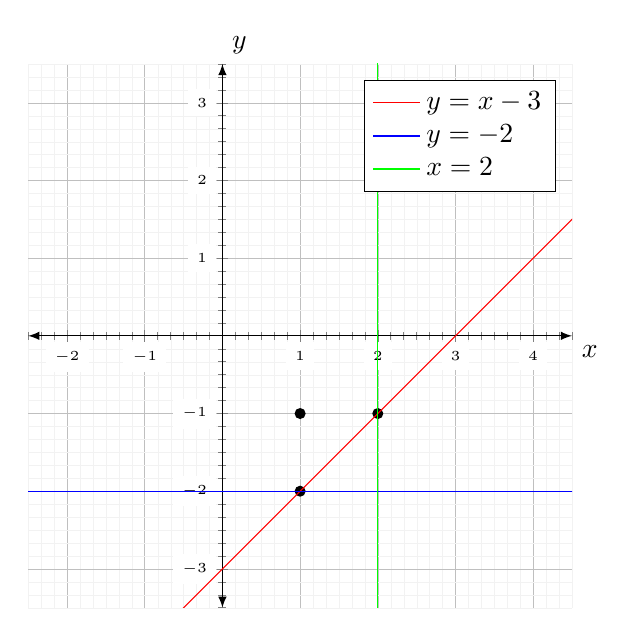
\begin{tikzpicture}
			\begin{axis}[
					width=0.7\textwidth,
					height=0.7\textwidth,
					xtick distance=1,
					ytick distance=1,
					xmin=-2.0,xmax=4,
					ymin=-3.0,ymax=3,
					xlabel = $x$,
					ylabel = $y$,
					grid=both,
					grid style={line width=.1pt, draw=gray!10},
					major grid style={line width=.2pt,draw=gray!50},
					axis lines=middle,
					minor tick num=5,
					enlargelimits={abs=0.5},
					axis line style={latex-latex},
					ticklabel style={font=\tiny,fill=white},
					xlabel style={at={(ticklabel* cs:1)},anchor=north west},
					ylabel style={at={(ticklabel* cs:1)},anchor=south west},
					legend pos=north east,
					legend entries={
						$y = x - 3$,
						$y = -2$,
						$x = 2$,
					},
					legend cell align={left},
				]
				\fill (axis cs: 1, -1) circle[radius=2pt];
				\draw (axis cs: 1, -1) circle[radius=100]; 
				
				\fill (axis cs: 1,	-2) circle[radius=2pt];
				\fill (axis cs: 2,	-1) circle[radius=2pt];

				\addplot[
					domain=-6:6, 
					samples=100, 
					color=red,
				]
				{ x - 3 };
				\addplot[
					domain=-6:6, 
					samples=100, 
					color=blue,
				]
				{ -2 };
				\addplot[color=green] table[row sep = crcr]{2 -5 \\ 2 5 \\};
			\end{axis}
		\end{tikzpicture}
	\end{center}
		
\end{solution}

\appenddata{questionSolutions}{
{
	The points of intersection are $(1, -2)$ and $(2, -1)$. 
	The tangents are $y = -2$ and $x = 2$ respectively. 
	They intersect at the point $(2, -2)$
}
}